\documentclass[12pt,a4paper]{standalone}
\usepackage[utf8]{inputenc}
\usepackage{amsmath}
\usepackage{amsfonts}
\usepackage{amssymb}
\usepackage{graphicx}
\newcommand*{\eps}{0.05}
\newcommand*{\Real}{\,\text{Re}}
\usepackage{tikz}
\usepackage{pgfplots}
\pgfplotsset{compat=newest}
\usetikzlibrary{decorations.markings}
\begin{document}

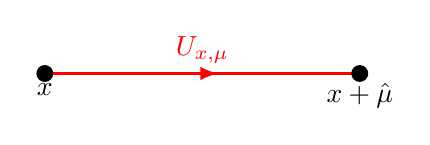
\begin{tikzpicture}
		\tikzset{middlearrow/.style={decoration={markings,mark= at position 0.55 with {\arrow{#1}} ,},postaction={decorate}}};
		\draw[middlearrow={latex}, very thick,red] (0,0)--(4,0);
		\draw[red] (2,0) node[above] {$U_{x,\mu}$};
		\filldraw[black] (0,0) circle(0.1) node[below]{$x$};
		\filldraw[black] (4,0) circle(0.1) node[below]{$x+\hat{\mu}$};
	\end{tikzpicture}




	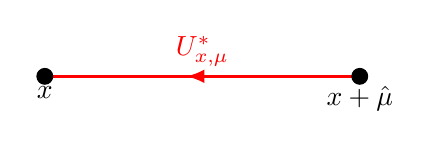
\begin{tikzpicture}
		\tikzset{middlearrow/.style={decoration={markings,mark= at position 0.55 with {\arrow{#1}} ,},postaction={decorate}}};
		\draw[middlearrow={latex}, very thick,red] (4,0)--(0,0);
		\draw[red] (2,0) node[above] {$ U^{*}_{x,\mu}$};
		\filldraw[black] (0,0) circle(0.1) node[below]{$x$};
		\filldraw[black] (4,0) circle(0.1) node[below]{$x+\hat{\mu}$};
	\end{tikzpicture}
	
\end{document}